\label{ch:fs}

Every day we work with various files, such as pictures, texts, or music.
For example, we search for them through directories, open them, modify them, close them, delete them, then remove them from the Recycle Bin because we deleted them by mistake, and so on.

Files are, thus, the most visible and used part of the operating system.
We want to have quick and easy access to files, to be able to locate them quickly and store as much data as possible.
These needs lead to the need for file organization.
To allow quick search and easy operations with files, they are organized in a hierarchical structure, called a \textbf{file system}.

\section{Basic Concepts}
\label{sec:data-files:concepts}

The file system is one of the central components of the operating system, which helps us organize impressive amounts of information, processes, and collaborators.
The file system has two important roles in the operating system:

\begin{itemize}
  \item First, it offers the possibility of \textbf{controlling an ever-increasing amount of documents}, allowing us to find a specific file among thousands, millions, or even billions of other files, in distributed systems.
    This contribution is detailed in \labelindexref{Section}{sec:data-files:filesystem} regarding the hierarchical structure.
  \item Second, file systems \textbf{ensure separation of resources between multiple users of a computing system}, whether human or non-human.
    We will discuss the importance of this feature in \labelindexref{Section}{sec:user:fs-access} dedicated to permissions.
\end{itemize}

File systems are diverse, \textbf{built and optimized for different usage contexts}.
There is no file system that is optimal for everyone.
To choose a file system, we need to know what the priorities are in the system's operation.
For example, the growth of storage resources has led to the disappearance of space crises and compression issues in personal systems;
however, this is increasingly relevant in \textit{cloud} architectures.
Nowadays, a user stores and uses movies, pictures, computer games, documents, virtual machines, information archives;
these occupy considerable space on a laptop system or on a smart mobile device or in Dropbox;
however, this occupied space is no longer considered a problem given the state of storage technologies and services.

Also, the requirements for data to be intact and valid (not corrupted) is very important in systems that work with critical data, but less important in personal systems, which need more simplicity and flexibility.
Among the criteria by which we can compare and choose file systems are:

\begin{itemize}
  \item ensuring data integrity;
  \item efficient separation of resources between different users;
  \item securing data by setting differentiated access permissions;
  \item managed volume: ease of working with very large files or with a very large number of files;
  \item file compression (\textit{file compression}) to maximize storage space on disk (compression means that the same data will occupy less space, but will require processor effort to decompress them on each use);
  \item optimizing storage space by managing duplicate files and inefficiently written areas on disk;
  \item managing possible errors through logging and reversibility, i.e., maintaining a list of changes that allows returning to a previous state in case of an error.
\end{itemize}

\subsection{Definitions}
\label{sec:data-files:defs}

We know, intuitively, what files are: they are our electronic documents, such as pictures, songs, college projects, or executable programs.

\textbf{File}: A file represents a form of digital organization of information, having the form of a sequence of bytes.

Information is organized in \textbf{files} for their use through an application and for their long-term storage.
Besides files created by human users, there are also files created by automated users.
Some of these are essential for the operation of the computing system and are hidden from regular users.

Files are organized in turn in \textbf{directories}.

\textbf{Directory}: A directory (\textit{folder} or \textit{directory}) represents a collection of files and subdirectories, identified by a name.

If we can understand a file by analogy with a \textbf{sheet} on which information is written, we can understand a directory by analogy with a \textbf{folder} that contains sheets of paper but also other folders.
A directory, like a folder, can also be empty.

This analogy is useful but can also be misleading.
From a technical perspective, directories are also files.
They do not actually "contain" the files they organize, as a folder contains sheets, but only their names - being similar to a sheet on which we have written a list of documents.
Therefore, directories in Linux are special files that serve to organize other files and directories.

\textbf{Note:} The more general concept of directory (\textit{folder}), taken from English and in our language, can refer to forms of information organization that have no equivalent in the file system.
For example, email interfaces may allow organizing messages in \textit{folders}.
These will not be found in the hierarchical structure of the file system, remaining accessible only through the interface in which they were created.

Files represent digital information inscribed on physical storage media (hard disk, USB stick, DVD, etc.).
Storage media can be considered continuous spaces of bytes, on which we can inscribe many files, of variable sizes.
To be able to read or write files on a storage medium, it is necessary to know the file system used for organizing it.

\textbf{File System}: The \textbf{file system} is a part of the operating system that deals with the names and attributes of files, storing them in a hierarchical structure.
The file system offers a method of physical and logical organization of files in a storage medium:

\begin{itemize}
  \item storing files as a sequence of bytes represents physical organization;
  \item the way files are addressed represents logical organization.
\end{itemize}

The file system thus helps the user store and organize digital data for easy access.
\labelindexref{Figure}{fig:data-files:def-fs} presents the role of the file system in organizing data;
the organization is usually hierarchical as presented in \labelindexref{Section}{sec:data-files:filesystem}.

\begin{figure}[htbp]
  \centering
  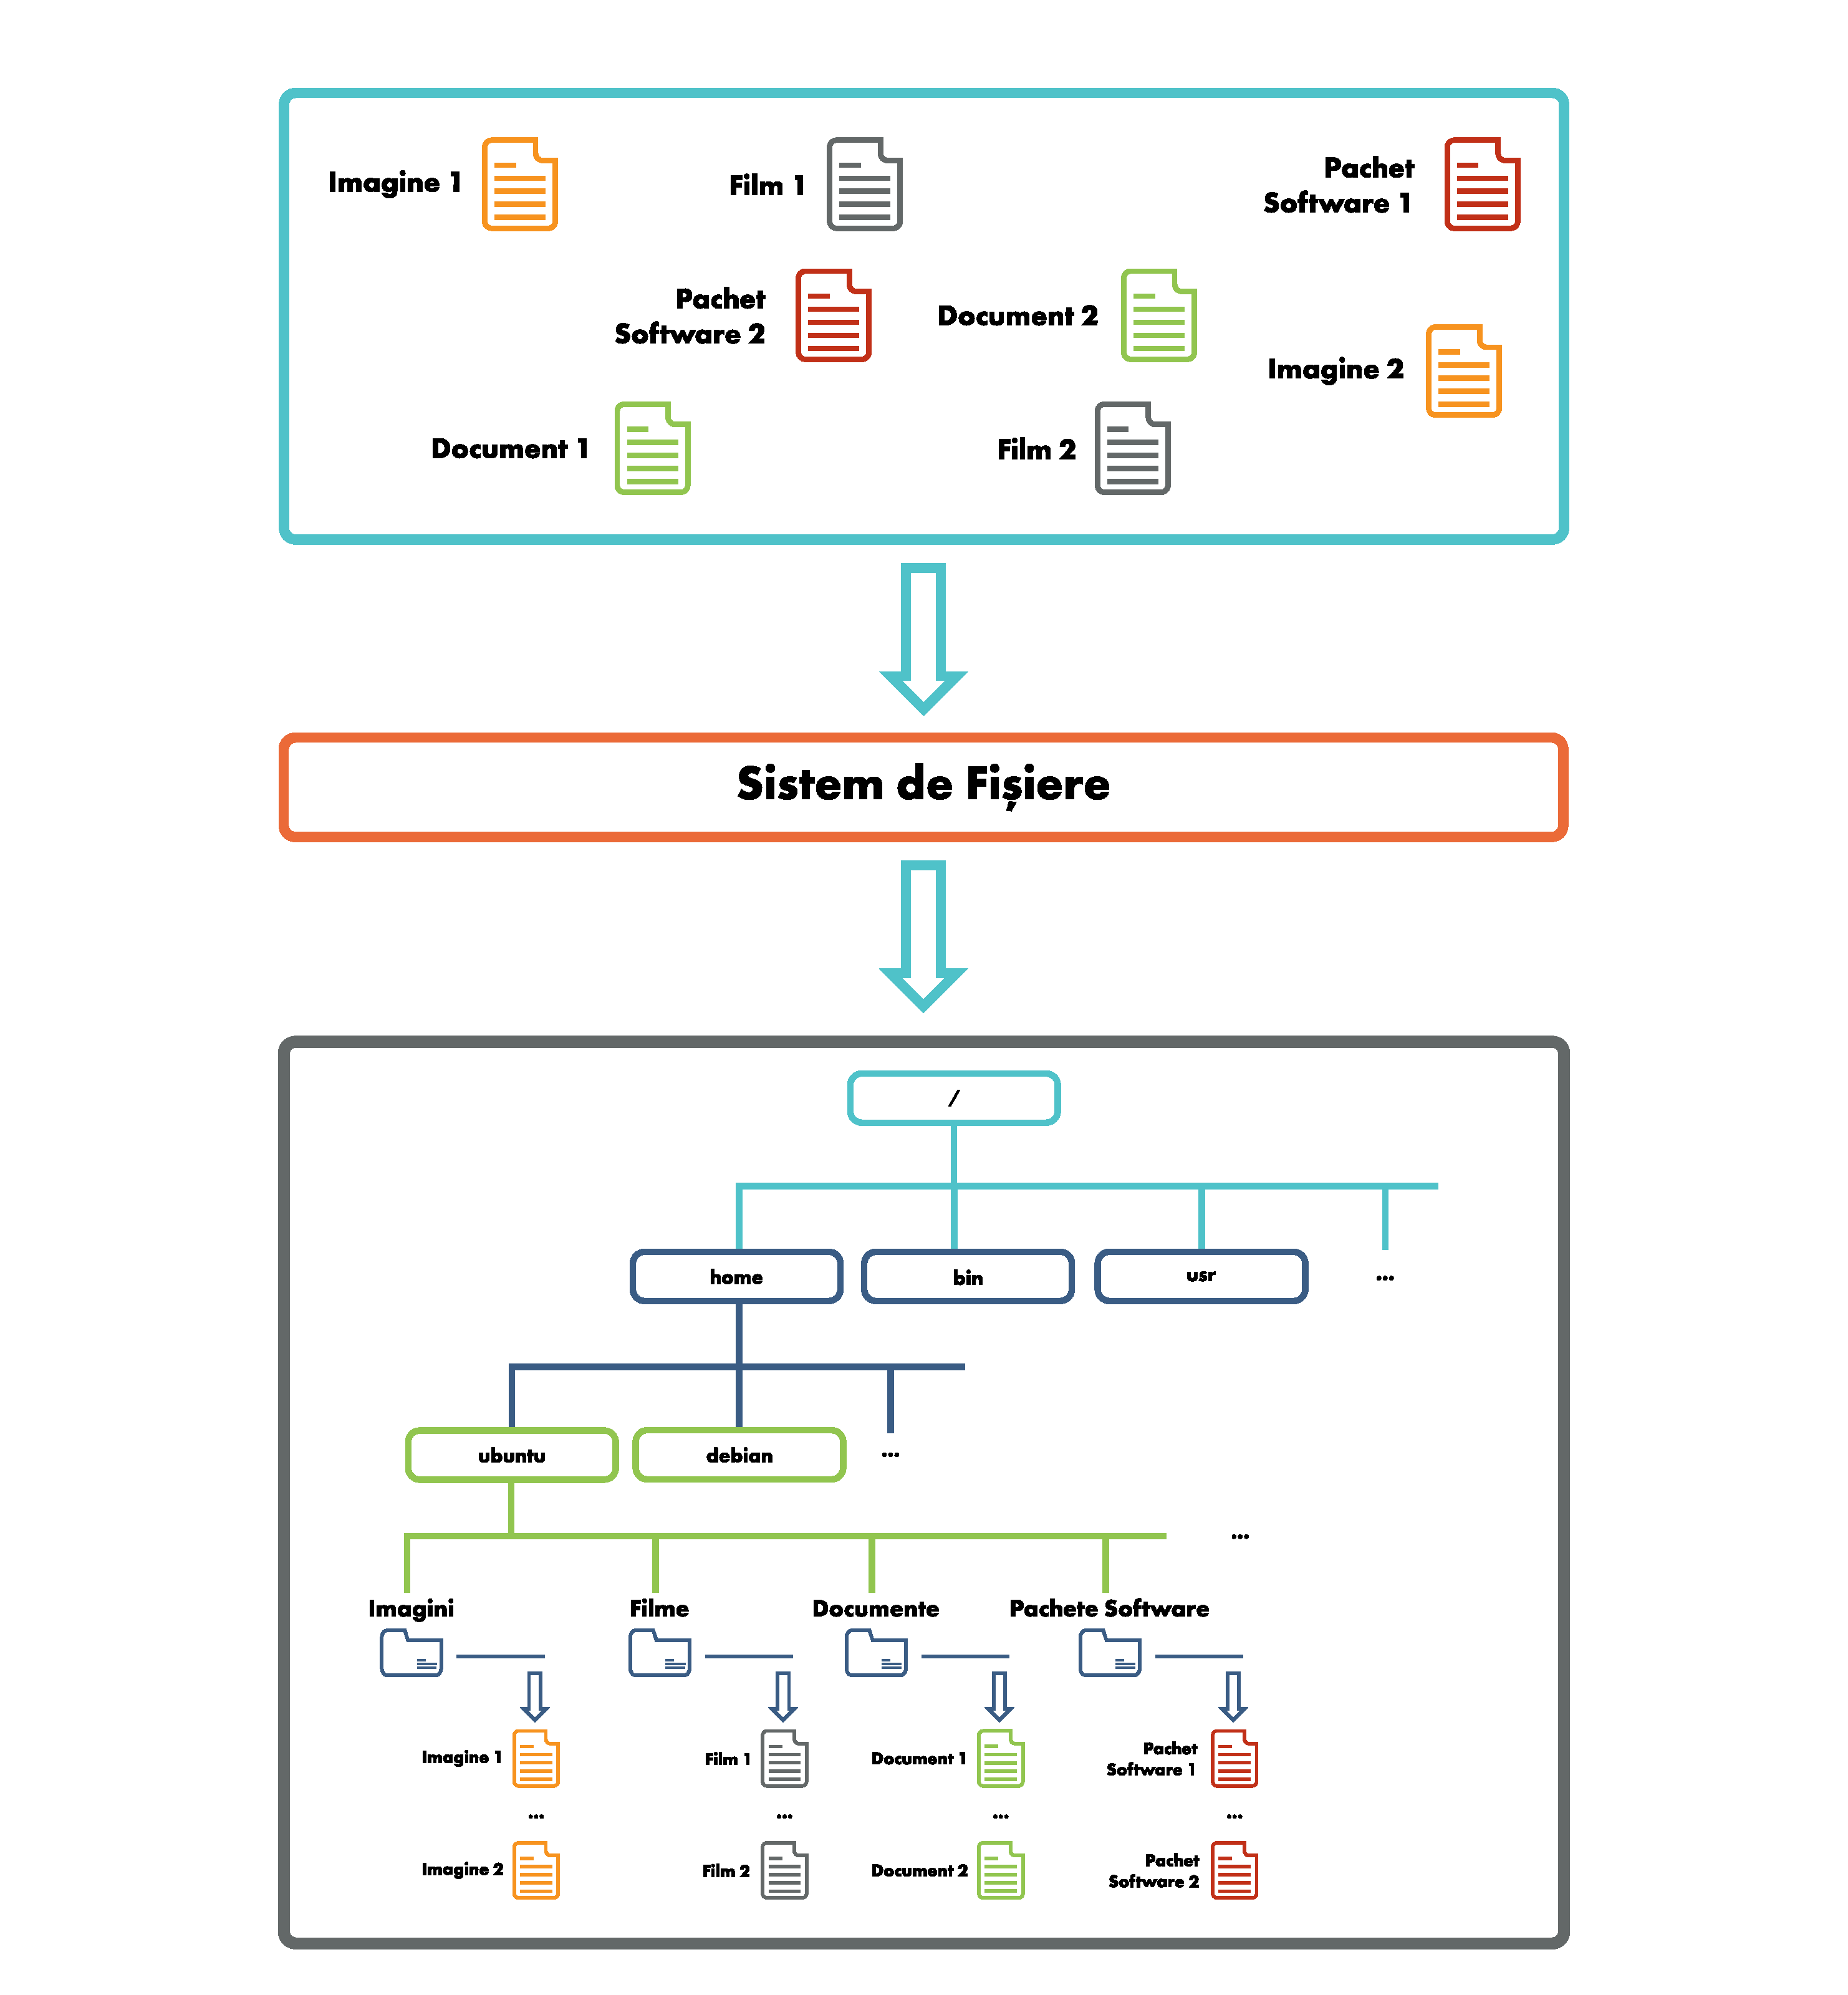
\includegraphics[width=0.5\columnwidth]{chapters/03-data-files/img/def-fs.pdf}
  \caption{The file system as organizer of digital data}
  \label{fig:data-files:def-fs}
\end{figure}

Files are used by the operating system to organize both data from the user and that generated by the system.
In the file system are stored and organized pictures, documents, user notes, but also configuration files, log files (\textit{log files}), databases necessary for system operation.

Since it is important that users can access stored files, the operating system provides an interface to work with the file system.
Depending on preferences, there are two types of interfaces, as described in \labelindexref{Chapter}{ch:ui}: the command line interface (CLI) exposed by the command interpreter (CLI shell) and the graphical interface (GUI) presented, for example, by a file system browser.

\subsection{Hierarchical Structure of the File System}
\label{sec:data-files:filesystem}

Year after year we have more and more files on computers and phones.
We accumulate pictures, videos, songs, as well as documents from school or office.
What would it mean to find a picture in a collection of one million pictures? The file system offers a hierarchical interface that allows organizing and searching for information.

A \textbf{hierarchical}, or tree-like, structure appears when files are organized in directories (\textit{folders}).
A directory can contain multiple files but also other directories, each of which can contain multiple files but also other directories and so on, until the last directory will contain only files or will be empty.
A directory is analogous to a branch of a tree, on which other branches can grow but also leaves (files).
Nothing grows on leaves.

Let's examine the following example.
To find a specific picture (for example, \file{selfiecumotanul-mai2018.jpg}) in a collection of 1,000,000 pictures, the user would have to ask the file system to go through all pictures until it finds the searched file name.
In the worst case, it would have to go through all 1,000,000 names.

What happens, however, if we resort to a three-level organization, grouping pictures by 100, as in \labelindexref{Figure}{fig:data-files:ex-3-lvl}? On the first level, we will have 100 directories.
In each of them, we include 100 subdirectories.
Then, in each subdirectory we include 100 pictures.
Thus, we have stored in a three-level hierarchy \texttt{100 directories * 100 subdirectories * 100 pictures = 1,000,000 pictures}.

\begin{figure}[htbp]
  \centering
  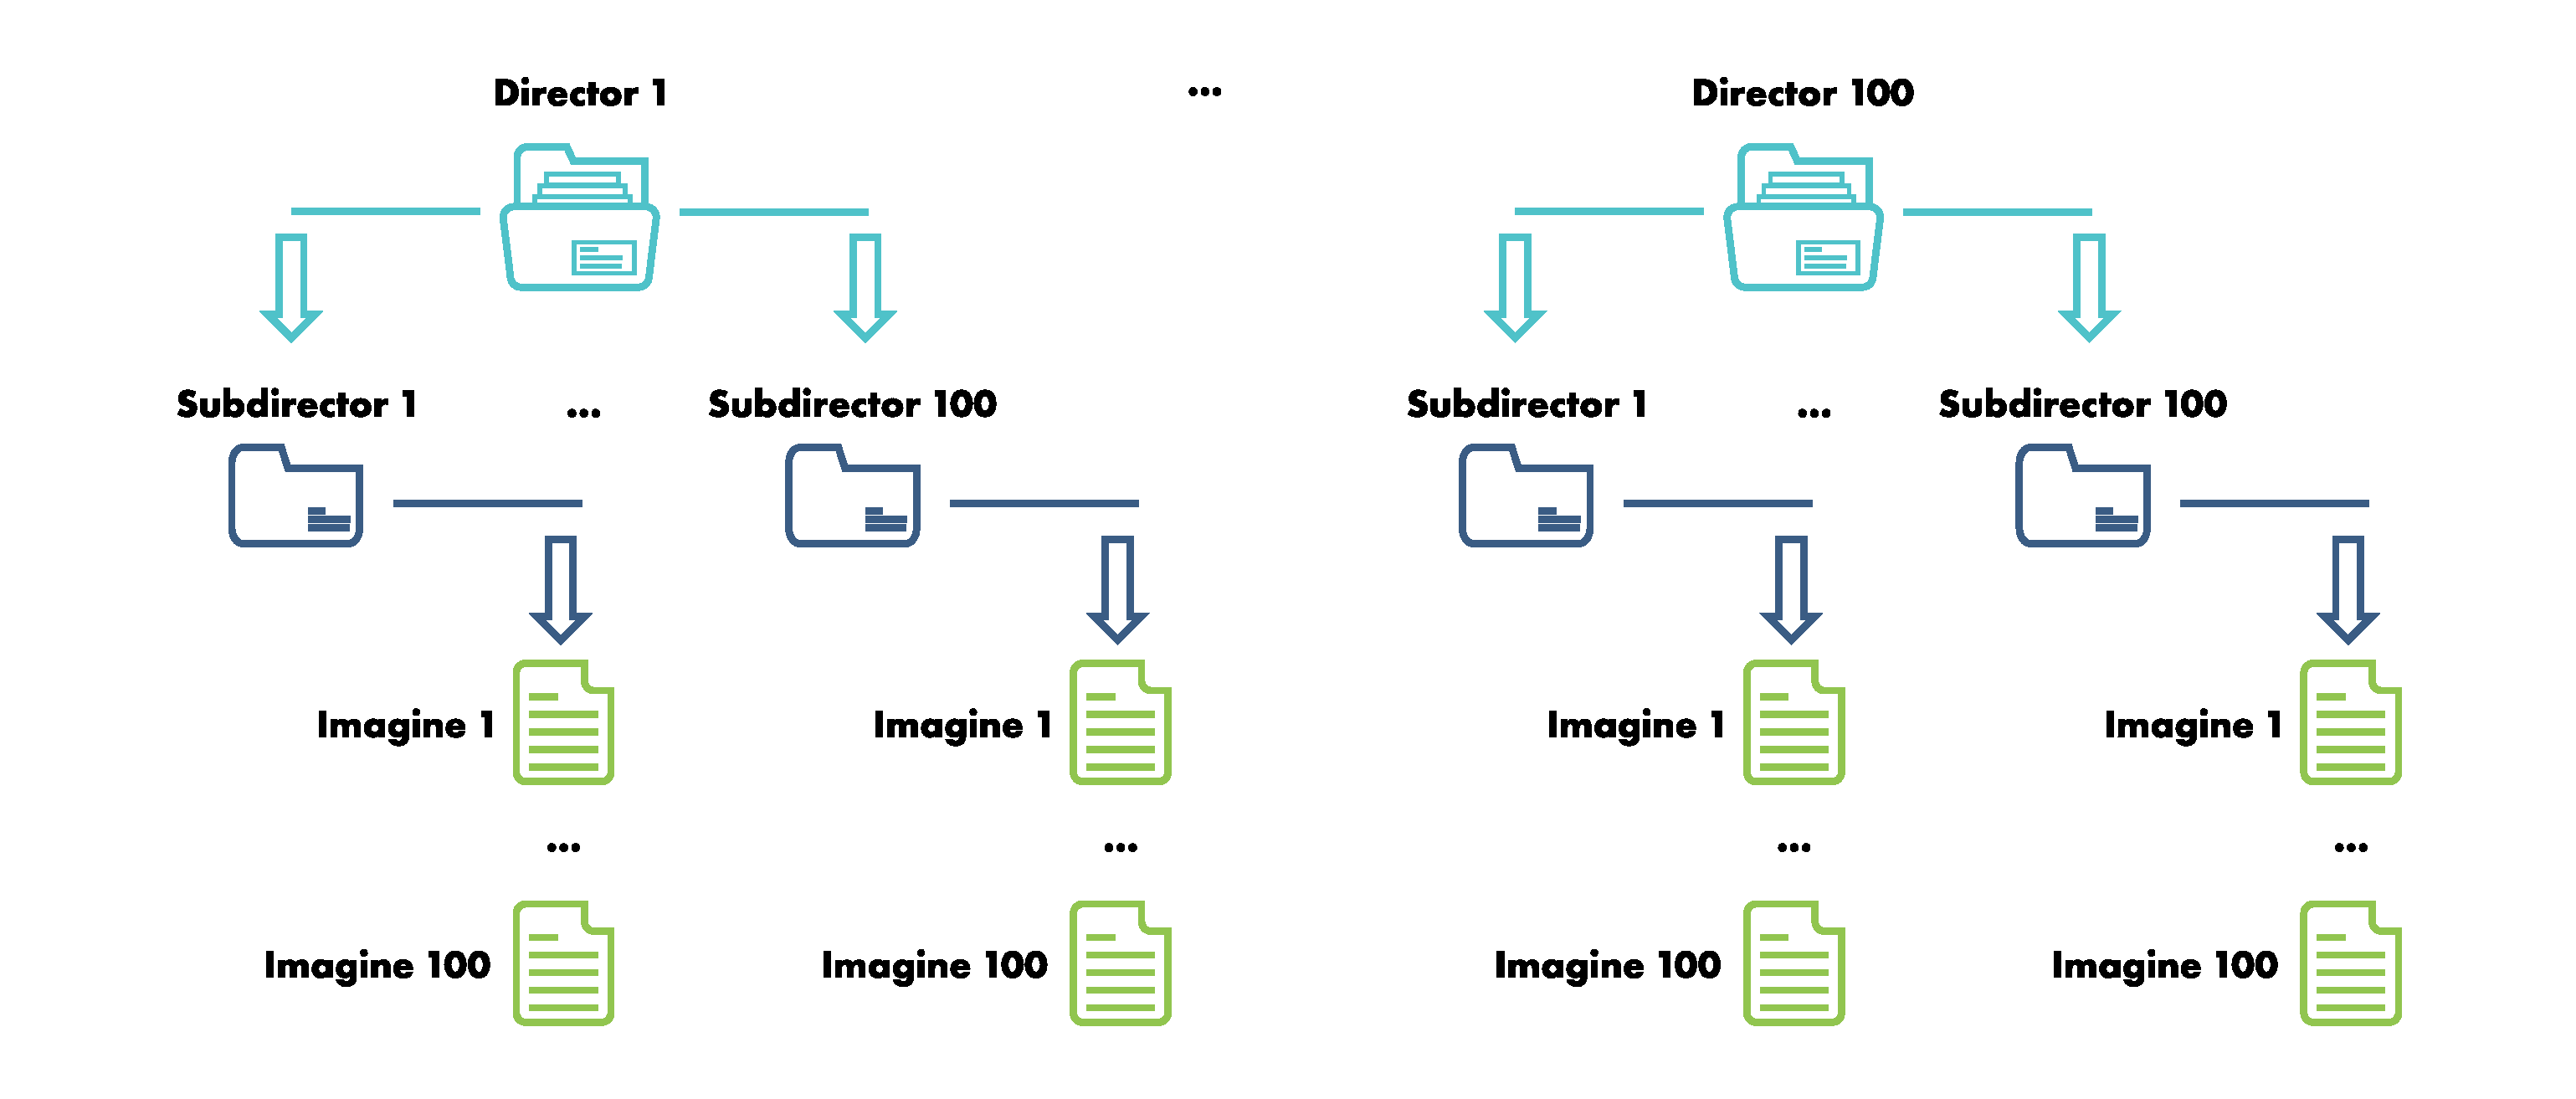
\includegraphics[width=\columnwidth]{chapters/03-data-files/img/3-lvl-fs.pdf}
  \caption{Example of three-level hierarchical organization of a set of 1,000,000 pictures}
  \label{fig:data-files:ex-3-lvl}
\end{figure}

How can we find the picture now? Its address will indicate where exactly it is located in the file tree.
For example, if its complete address is: Directory \file{99/cat-pics/selfiecumotanul-mai2018.jpg}, the file system will first search for directory \file{99} among the 100 directories on the first level.
Then, it will search for \file{cat-pics} among the 100 subdirectories in directory 99.
Then, finally, it will search for the desired picture.
In the worst case, the file system will perform, three times in a row, a search among 100 elements.

Through the three-level tree structure, we have thus replaced a search in a bag with 1,000,000 elements, which one person accomplishes in hours if not days, with a search in three small bags with 100 elements each, which is easy to accomplish even manually, by one person.

Through tree organization by directories, a large number of files can be managed at the level of a single person.
The file system thus transforms the complexity of the immense volume of information and makes it accessible to the human user.
More about finding files is in \labelindexref{Section}{sec:file-mgmt:search} regarding search commands (\cmd{find}, \cmd{locate}, \cmd{whereis}, \cmd{which} and \cmd{type}).

However, there is a cost for this increased control of complexity.
Each directory is an additional element, created by the file system, which must also be stored somewhere and thus occupies resources.
These directories do not exist in the flat structure, where we thus save space.
In the above example, in the hierarchical structure we have a total of 100*100=10,000 directories, created specifically to organize the 1,000,000 pictures.
Therefore, relative to the initial number of files, to better control information we pay a cost of 10,000 / 1,000,000 = 1\%.

We present below concrete examples of file organization in modern operating systems.

In \labelindexref{Table}{table:data-files:linux-fs} the hierarchical structure in Linux is presented.

\begin{table}[!htb]
  \begin{center}
    \begin{tabular}{ p{0.2\textwidth} p{0.7\textwidth} }
      \hline
        \textbf{Directory} &
        \textbf{Content} \\
      \hline
        \file{/} &
        root directory (\textit{root directory}) -- the most comprehensive directory, which contains the other directories, considered analogous to trunk and branches \\
      \hline
        \file{/bin} &
        essential commands necessary for booting, maintenance and debugging the system \\
      \hline
        \file{/boot} &
        files necessary for booting, such as the kernel image \\
      \hline
        \file{/dev} &
        special files used for direct access to hardware or logical devices of the system \\
      \hline
        \file{/etc} &
        files for system configuration, such as \file{inittab}, \file{fstab} and \file{hosts} \\
      \hline
        \file{/home} &
        files of each user in the system - a user's data is found in \file{/home/username} \\
      \hline
        \file{/media} &
        subdirectories where optical units, floppy disks etc. are mounted \\
      \hline
        \file{/mnt} &
        subdirectories where other file systems are mounted \\
      \hline
        \file{/opt} &
        large application packages, accessible to all users \\
      \hline
        \file{/proc} &
        virtual file system from which information about the system and applications running at a given time is obtained \\
      \hline
        \file{/root} &
        home directory of the root user \\
      \hline
        \file{/sbin} &
        basic commands accessible only to the root user \\
      \hline
        \file{/tmp} &
        temporary files \\
      \hline
        \file{/usr} &
        applications for normal use of the operating system - \file{/usr/local} contains applications installed/compiled by the user \\
      \hline
        \file{/var} &
        files whose content changes very often, such as logs, temporary files, cache (reusable data), spool (unprocessed data) \\
      \hline
    \end{tabular}
  \end{center}
  \caption{Hierarchy in a Linux file system}
  \label{table:data-files:linux-fs}
\end{table}

In \labelindexref{Figure}{fig:data-files:linux-fs} we present how a file system hierarchy looks graphically.
We observe that in the root are the directories \file{home/}, \file{bin/}, \file{usr/} etc.
In the \file{home/} directory are the subdirectories \file{ubuntu/} and \file{myuser/} etc.

\textbf{Note:} When we use directory names in Linux we will prefer to use the suffix \texttt{/} (\textit{slash}) to indicate that they are directories.

\begin{figure}[htbp]
  \centering
  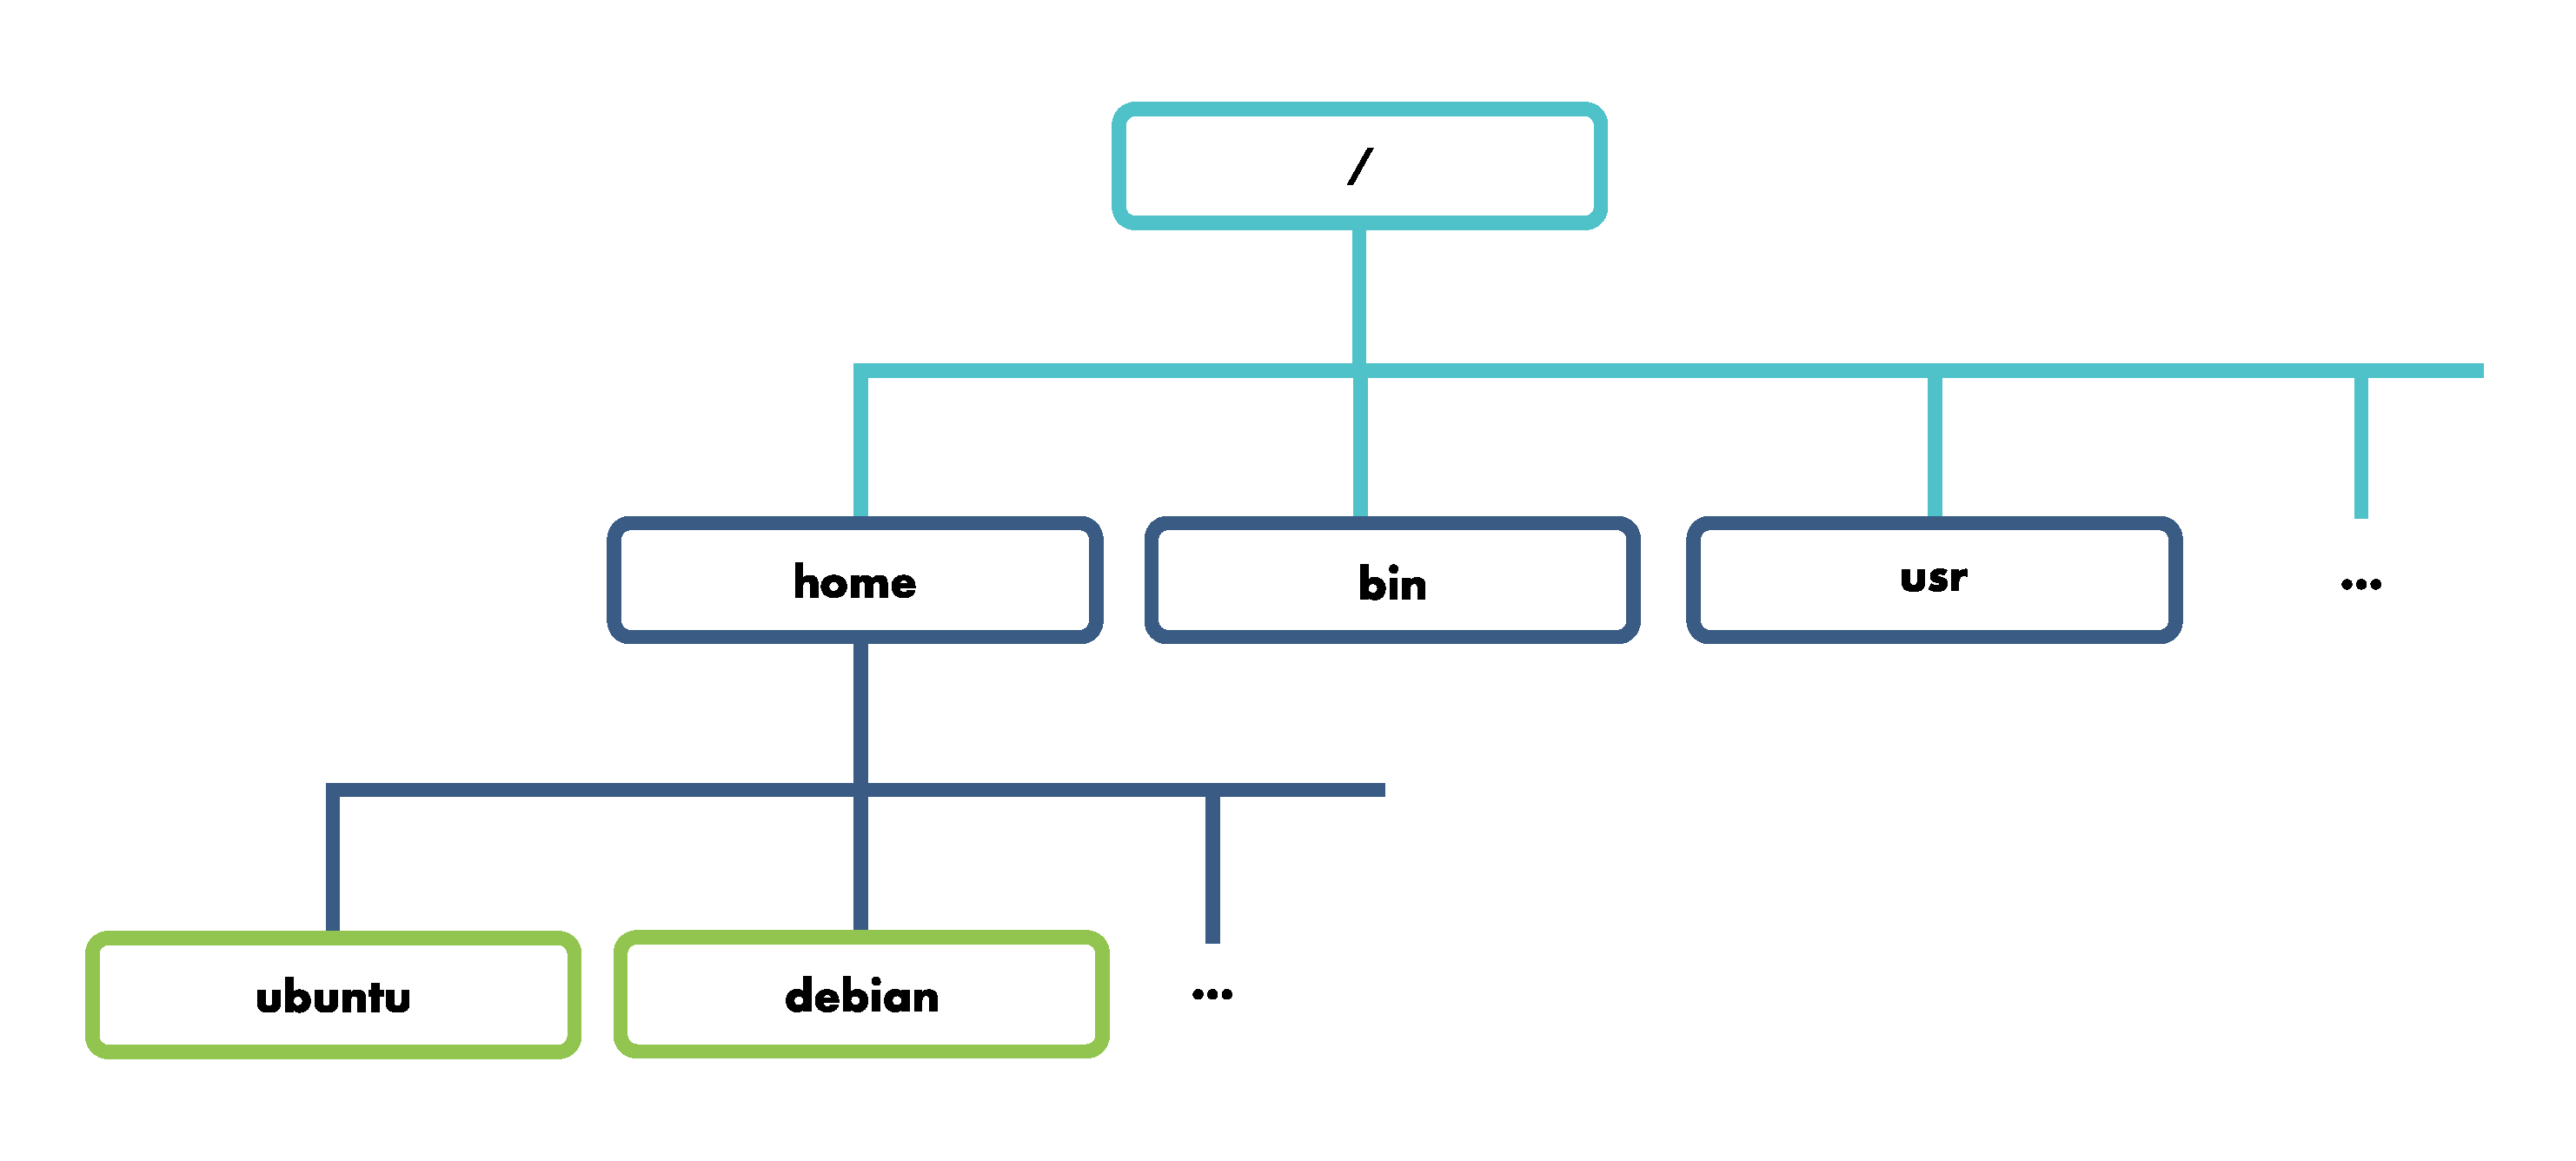
\includegraphics[width=0.7\columnwidth]{chapters/03-data-files/img/linux-fs.pdf}
  \caption{Hierarchy in a Linux file system}
  \label{fig:data-files:linux-fs}
\end{figure}

The file system hierarchy in macOS is similar to that in Linux.

The file structure in Windows differs from that in Linux.
This is simpler and most important directories are in \file{C:\textbackslash{}Windows}, as observed in \labelindexref{Table}{table:data-files:windows-fs}.

\begin{table}[htb]
  \begin{center}
    \begin{tabular}{ p{0.32\textwidth} p{0.62\textwidth} }
      \hline
        \textbf{Directory} &
         \textbf{Content} \\
      \hline
        \file{C:\textbackslash{}} &
        root directory \\
      \hline
        \file{C:\textbackslash{}Windows} &
        Windows and related files \\
      \hline
        \file{C:\textbackslash{}Documents and Settings} &
        user configurations and their specific data \\
      \hline
        \file{C:\textbackslash{}Program Files} &
        applications \\
      \hline
        \file{C:\textbackslash{}Windows\textbackslash{}System32} &
        Windows drivers and configuration files \\
      \hline
        \file{C:\textbackslash{}Documents and Settings\textbackslash{}username\textbackslash{}My Documents} &
        user data (this is the default path, it can be modified) \\
      \hline
    \end{tabular}
  \end{center}
\caption{Hierarchy in a Windows file system}
\label{table:data-files:windows-fs}
\end{table}

Although in Linux and macOS we have a single root directory, Windows has simultaneously for each file system a root directory:

\begin{itemize}
  \item \file{A}, \file{B}: are usually reserved for floppy disks;
  \item \file{C}: hard disk partition;
    there can be more, to which letters are associated in order;
  \item \file{D} (or the next available letter after hard disk partitions): refers to CD-ROM/DVD-ROM.
\end{itemize}

Windows allocates letters based on partitions, not by file system.
If the file system on a partition is changed, the letter assigned to the partition will remain the same.
On a partition there can be at one time only one file system.

In \labelindexref{Table}{table:data-files:compare-lin-win} below we have a comparison between important paths in the most known operating systems.

\begin{table}[htb]
  \scriptsize
  \begin{center}
    \begin{tabular}{ p{0.15\textwidth} p{0.25\textwidth} p{0.25\textwidth} p{0.25\textwidth} }
      \hline
        \textbf{Description} &
        \textbf{Windows} &
        \textbf{Linux} &
        \textbf{Mac OS} \\
      \hline
        root &
        \file{C:} &
        \file{/} &
        \file{/} \\
      \hline
        home directory &
        \file{C:\textbackslash{}Documents and Settings\textbackslash{}username} &
        \file{/home/username} &
        \file{/Users/username} \\
      \hline
        applications &
        \file{C:\textbackslash{}Program Files} &
        \file{/bin}; \file{/sbin}; \file{/usr/bin}; \file{/usr/sbin}; \file{/usr/local/bin}; &
        \file{/opt/*/bin} \file{/Applications}; \file{/bin}; \file{/sbin} \\
      \hline
        system configurations &
        Windows Registry &
        specific directories for each application, located in the user's home; \file{/etc} &
        \file{/Users/username/ Library}; \file{/etc} \\
      \hline
    \end{tabular}
  \end{center}
  \caption{Comparison between operating system paths}
  \label{table:data-files:compare-lin-win}
\end{table}

We observe that in Linux the sequence of directories is separated by the character \file{/} (\textit{slash}), while in Windows environments \file{\textbackslash{}} (\textit{backslash}) is used.

\subsection{Relative and Absolute Paths}
\label{sec:data-files:path}

Returning to the example from \labelindexref{Figure}{fig:data-files:linux-fs}, we want to find the picture \file{selfiecumotanul-mai2018.jpg}, which is in the subdirectory \file{cat-pics}, in directory \file{99}.
To be able to access the picture, we have two possibilities: we can use a relative path or an absolute path.
The choice of path we will use depends on where we are at that moment in the file hierarchy and where the searched file is located.
A path is the equivalent of an address for identifying the file.

\textbf{Absolute Path}: An \textbf{absolute path} represents the complete address of the file, starting with the root directory.
Thus, an absolute path will start with \file{/} (\textit{slash}) or \file{\textasciitilde{}} (tilde, \textit{tilde}) in the case of Linux/macOS or with \file{C:}, \file{D:} etc, in the case of Windows.

\textbf{Relative Path}: A \textbf{relative path} is a path that starts from the current directory.
Starting from the current directory, a path to the desired destination file is constructed.
A relative path \textbf{does not} start with \file{/} (\textit{slash}) or \file{\textasciitilde{}} (tilde, \textit{tilde}) in the case of Linux/macOS or with \file{C:}, \file{D:} etc, in the case of Windows.

\textbf{Note:} The symbol \file{\textasciitilde{}} is an abbreviation in Linux/macOS for the user's \textit{home} directory.
Usually this is \file{/home/$<$username$>$/} in Linux and \file{/Users/$<$username$>$/} in macOS.

In each directory there are \textbf{two special directories}: \file{.} (dot) and \file{..} (dot dot).
The directory \file{.} (\textit{dot}) points to the same directory, the current directory.
\file{..} (\textit{dot dot}) points to the parent directory in the file and directory hierarchy.

To go back in the file hierarchy step by step, we use \file{..} to reach the parent directory.
We can chain multiple \file{..} groupings (e.g. \file{../../..}) to go back higher in the hierarchy.
We have an example of commands in \labelindexref{Listing}{lst:data-files:dot-dot}.

\begin{screen}[style=bashstyle][style=bashstyle,caption={Reference .. to parent directory},label={lst:data-files:dot-dot}]
student@uso:~$ pwd
/home/student
student@uso:~$ cd uso.git/labs/
student@uso:~/uso.git/labs$ pwd
/home/student/uso.git/labs
student@uso:~/uso.git/labs$ cd ..
student@uso:~/uso.git$ pwd
/home/student/uso.git
student@uso:~/uso.git$ cd ../..
student@uso:/home$ pwd
/home
student@uso:/home$ cd
student@uso:~$ pwd
/home/student
student@uso:~$ cd /usr/local
student@uso:/usr/local$ pwd
/usr/local
\end{screen}

In the above example we used the \cmd{pwd} command (\textit{print working directory}) to display the current directory (also called working directory).
The directory is also indicated in the command prompt, between the \texttt{:} character (colon) and the \texttt{\$} character (dollar);
the \texttt{$\sim$} symbol (tilde) is equivalent to the user's home directory, in the above case \texttt{/home/student/}.
The \cmd{cd} command (\textit{change directory}) changes the current directory;
the command receives as argument a path that can be relative or absolute.

At line 6 in the above example we changed the working directory to the parent directory using the \cmd{cd ..} command and went up one level in the directory hierarchy;
we observe that a shorter path is displayed at line 8 (\file{/home/student/uso.git}) compared to the previous path at line 5 (\file{/home/student/uso.git/labs}).
At line 9 is a relative path (\file{../..}) that goes up two levels in the hierarchy.
At line 12 we have the \cmd{cd} command without arguments;
this use of the command changes the working directory to the user's home directory, in our case \file{/home/student/}.
At line 15 we have an absolute path (which starts with \texttt{/} (\textit{slash})): \file{/usr/local};
the \cmd{cd} command receives this path as argument and changes the current directory to \file{/usr/local}.

So far we have presented only when we use the special directory \file{..} (dot dot).

Often, we use the \file{.} (dot) construction, which indicates the current directory, for commands that execute scripts/programs from that directory.
If in the current directory we have an executable named \texttt{list\_permissions}, then we can run it using the command:

\begin{screen}[style=bashstyle]
student@uso:~$ ./list_permissions
\end{screen}

This means to execute the executable \file{list\_permissions} from the current directory.

The \file{.} (dot) construction can be used in situations where we want to refer to the current directory.
For example, if we want to copy a file to the current directory, we run a command similar to that on line 5 in \labelindexref{Listing}{lst:data-files:dot}.

\begin{screen}[style=bashstyle][caption={Reference . to current directory},label={lst:data-files:dot}]
student@uso:~$ pwd
/home/student
student@uso:~$ ls
Desktop  Documents  Downloads  Music  Pictures  Public  Templates  Videos  examples.desktop  uso.git  vm-actions-log.txt
student@uso:~$ cp /etc/passwd .
student@uso:~$ ls
Desktop  Documents  Downloads  Music  Pictures  Public  Templates  Videos  examples.desktop  passwd  uso.git  vm-actions-log.txt
\end{screen}

In the above example we used the \cmd{ls} command (\textit{list}) to display the content of the current directory (even the home directory \file{/home/student}).
Then, at line 5 we used the \cmd{cp} command (\textit{copy}) to copy the file \file{/etc/passwd} (absolute path), given as the first argument, to the current directory, represented by the \file{.} (dot) construction, given as the second argument.
Then, when displaying the directory content (using the \cmd{ls} command) we see the presence of the \texttt{passwd} file, now copied.
In the example we used the \file{.} (dot) construction to refer to the current directory, the destination of the copy command.

\section{File Format}
\label{sec:data-files:file-format}

From the user's perspective, files are divided into various categories, such as music, pictures, games, and others.
All of these are seen by the computer as a collection of bits that must be processed to be able to be reproduced.
The computer processes files according to their \textbf{format}, to know what programs are necessary to be able to open them and work with them.

To begin with, we can classify files into two major categories: text files (\textit{text file}) and binary files (\textit{binary file}).

\begin{itemize}
  \item \textbf{Text files} contain lines composed of readable characters (letters, digits, punctuation marks) without containing elements that must be interpreted by a program (such as graphics, executable code, etc.).
    Text files can contain plain text (\textit{plain text}), having the extension \texttt{.txt}, or which contain source code (for example with extension \texttt{.c} or \texttt{.java}) or presentation formats such as HTML.
  \item \textbf{Binary files} are all files that are not text type, and can represent: images, executable programs, songs, compressed files, etc.
\end{itemize}

The format (or type) of files refers to the way information is encoded in the file, which then allows the reproduction or use of information through an interface or application.
The file format specifies how the information will be encoded in bits, in the digital environment.

The file format is, as a rule, associated with its \textbf{extension}.
The extension represents the suffix at the end of the file name, separated from the file name by a dot.
Examples of extensions are: \texttt{.txt} (text files), \texttt{.tex} (LaTeX source document), \texttt{.mp3} (audio format), \texttt{.bmp} (bitmap image), \texttt{.png} (Portable Network Graphic image), etc.

It is important to note that, \textbf{if we manually change a file's extension, it doesn't mean we've changed its type}.
The file format depends on the properties of its content and does not change if we modify the name or extension.
If, for example, we have a text file in which we put the lyrics of the song "The Kinslayer" by the band Nightwish, and we change the file name from \file{kinslayer.txt} to \file{kinslayer.mp3}, the text file does not suddenly become a song and, of course, we will not be able to open it with an MP3 player application.

Files can be converted from one format to another, usually within the major content categories.
For example, we can convert a \texttt{.wav} file to an \texttt{.mp3} file, or a \texttt{.bmp} file to a \texttt{.png} file, or a \texttt{.doc} file to a \texttt{.pdf} file.
It is possible to convert files to formats that seem very different, for example a \texttt{.txt} file to an \texttt{.mp3} file, using automated text-to-speech solutions.
Conversion is done not by manually changing the extension, but through an application with which we open the file and transform it into the desired format.

To see what type a file is in Linux, beyond the extension, we use the \cmd{file} command.
Below we have examples of using the \cmd{file} command to determine the type of a file.
For each file received as argument by the \cmd{file} command, information about the file type is indicated: executable, kernel image, shell script, compressed file, image file.
\labelindexref{Listing}{lst:data-files:file} contains examples of running the \cmd{file} command.

\begin{screen}[style=bashstyle][caption={Finding the type of a file (file command)},label={lst:data-files:file}]
student@uso:~$ file /bin/ls
/bin/ls: ELF 64-bit LSB shared object, x86-64, version 1 (SYSV), dynamically linked, interpreter /lib64/ld-linux-x86-64.so.2, for GNU/Linux 3.2.0, BuildID[sha1]=9567f9a28e66f4d7ec4baf31cfbf68d0410f0ae6, stripped
student@uso:~$ file /boot/vmlinuz-4.15.0-29-generic
/boot/vmlinuz-4.15.0-29-generic: Linux kernel x86 boot executable bzImage, version 4.15.0-29-generic (buildd@lgw01-amd64-057) #31-Ubuntu SMP Tue Jul 17 15:39:52 UTC 2018, RO-rootFS, swap_dev 0x7, Normal VGA
student@uso:~$ file /etc/init.d/ssh
/etc/init.d/ssh: POSIX shell script, ASCII text executable
student@uso:~$ file /usr/share/man/man1/cp.1.gz
/usr/share/man/man1/cp.1.gz: gzip compressed data, max compression, from Unix
student@uso:~$ file /usr/share/pixmaps/htop.png
/usr/share/pixmaps/htop.png: PNG image data, 128 x 128, 8-bit/color RGBA, non-interlaced
\end{screen}

In \labelindexref{Listing}{lst:data-files:file} we analyzed five files using the \cmd{file} command and the following types resulted:
\begin{itemize}
  \item the file \file{/bin/ls} is an ELF (\textit{Executable and Linking Format}) executable \abbrev{ELF}{Executable and Linking Format}
  \item the file \file{/boot/vmlinuz-4.15.0-29-generic} is an operating system kernel image
  \item the file \file{/etc/init.ssh} is a shell script
  \item the file \file{/usr/share/man/man1/cp.1.gz} is a GZIP format compressed file
  \item the file \file{/usr/share/pixmaps/htop.png} is a PNG image file
\end{itemize}

The \cmd{file} command works independently of the file extension.
This is advantageous because the extension can be incorrectly assigned by the user, as we can see in \labelindexref{Listing}{lst:data-files:file-wrong-extension}.
Even though the file extension was changed from \texttt{.jpg} to \texttt{.txt}, the \cmd{file} command still detects the correct file type: JPEG image file.

\begin{screen}[style=bashstyle][caption={Detecting the type of a file with wrong extension},label={lst:data-files:file-wrong-extension}]
student@uso:~$ file photo.jpg
photo.jpg: JPEG image data, JFIF standard 1.01
student@uso:~$ mv photo.jpg fisier.txt
student@uso:~$ file fisier.txt
fisier.txt: JPEG image data, JFIF standard 1.01
\end{screen}

\subsection{File Attributes}
\label{sec:data-files:file-attr}

To control the operation of file systems, the distinction between \textbf{data} and \textbf{metadata} is important.
A file actually contains information or data, such as music, lyrics, images, or plane tickets.

\textbf{File Metadata}: \textbf{Metadata} is information about information: the amount of information, the date of last access, who created it, who modified it, where exactly it was last edited.

File systems are based on creating and managing metadata related to files.
This metadata is called \textbf{attributes}.
They make possible efficient and secure access to information.

In Linux we can display file attributes using the \cmd{ls} command with the \texttt{-l} option;
the option means \textit{long listing} and is used for detailed display (with file attributes), as in \labelindexref{Listing}{lst:data-files:long-listing}.
In \labelindexref{Listing}{lst:data-files:long-listing} we see on columns, file attributes, such as: permissions, ownership information (user), size, date of last modification, file name.

\begin{screen}[style=bashstyle][caption={Displaying file attributes (using ls)},label={lst:data-files:long-listing}]
student@uso:~$ ls -l
total 60
drwxr-xr-x  2 student student 4096 aug  6 17:41 Desktop
drwxr-xr-x  3 student student 4096 aug 20 21:00 Documents
drwxr-xr-x  2 student student 4096 aug  6 17:41 Downloads
drwxr-xr-x  2 student student 4096 aug  6 17:41 Music
drwxr-xr-x  2 student student 4096 aug  6 17:41 Pictures
drwxr-xr-x  2 student student 4096 aug  6 17:41 Public
drwxr-xr-x  2 student student 4096 aug  6 17:41 Templates
drwxr-xr-x  2 student student 4096 aug  6 17:41 Videos
-rw-r--r--  1 student student 8980 aug  6 17:37 examples.desktop
-rw-r--r--  1 student student 2506 sep 30 11:28 passwd
drwxr-xr-x 15 student student 4096 aug 24 14:52 uso.git
-rw-r--r--  1 student student 4827 aug 21 14:37 vm-actions-log.txt
\end{screen}

The simplest attributes of a file are name, size, and type.
The file type is indicated by the first character in the result of running the \cmd{ls -l} command, and can be:

\begin{itemize}
  \item \texttt{-} = regular file
  \item \texttt{b} = block special file
  \item \texttt{c} = character special file
  \item \texttt{d} = directory
  \item \texttt{l} = symbolic link
  \item \texttt{n} = network file
  \item \texttt{p} = FIFO
  \item \texttt{s} = socket
\end{itemize}

In the run from \labelindexref{Listing}{lst:data-files:long-listing} we have files (first character is \texttt{-}) and directories (first character is \texttt{d}).

Other important attributes describe permissions, i.e., operations that different types of users can perform on the respective file.
Detailed information about \textbf{user types} and configuring their permissions is found in \labelindexref{Chapter}{ch:user}.

\begin{itemize}
  \item \texttt{r} = permission to read the file
  \item \texttt{w} = permission to write to the file
  \item \texttt{x} = permission to execute the file
  \item \texttt{-} = absence of permission
\end{itemize}

\section{Summary}
\label{sec:data-files:summary}

Files represent some of the operating system components closest to the user.
The user uses files to retain their own information or because they are used by applications.

Files are organized in a hierarchical structure, for quick access.
The structure is called a file system.
At the top of the file system hierarchy is the root directory.
A file or directory is identified by a path in the file system.
The absolute path starts from the root directory.

The operating system provides utilities for performing common operations with files: creation, deletion, renaming, searching, displaying content, modifying content.
These operations are common to all operating systems and file systems.
